\begin{frame}{conclusion}{summary}
    %\vspace{-2mm}
		\begin{columns}
				\column{.6\linewidth}
						\begin{itemize}
								\item music analysis offers a \textbf{wide range of tasks} that require \textbf{specialized solutions} and \textbf{domain knowledge}
								
								\bigskip
								\item \textbf{training data} availability remains an open problem for many music tasks
								
								\bigskip
								\item \textbf{knowledge transfer} methodologies allow for compensating limited (and potentially biased) training data
						\end{itemize}
    		\column{.4\linewidth}
						\begin{figure}
								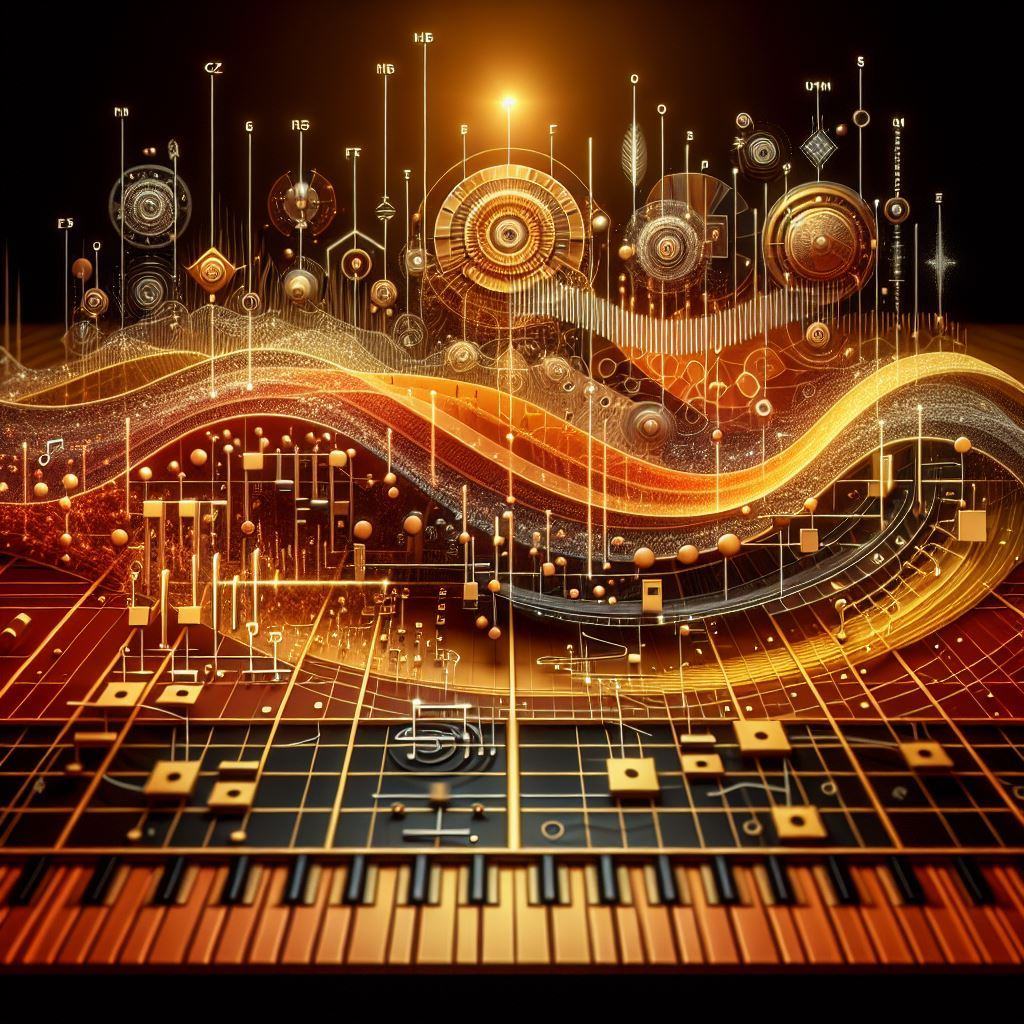
\includegraphics[width=.8\columnwidth]{music}
						\end{figure}
		\end{columns}
    \inserticon{lightbulb}
\end{frame}

\begin{frame}{conclusion}{future work}
    \vspace{-5mm}
		\begin{columns}
				\column{.6\linewidth}
						\begin{enumerate}
								\item \textbf{knowledge transfer }
										\begin{itemize}
												\item	transfer knowledge between tasks/modalities
												\item	inject expert knowledge
										\end{itemize}
								\smallskip
								
								\item \textbf{representation learning}
										\begin{itemize}
												\item interpretability of embedding spaces
												\item understanding of learned information
										\end{itemize}
										
								\smallskip
								\item \textbf{machine learning with insufficient data}
										\begin{itemize}
												\item 	approaches reducing the risk of overfitting
												\item 	lsynthesis and augmentation techniques
										\end{itemize}
										
								\smallskip
								\item \textbf{evaluation of generative systems}
										\begin{itemize}
												\item 	extendable framework for objective evaluation metrics
												\item 	detection of generated content
										\end{itemize}
						\end{enumerate}
    		\column{.4\linewidth}
						\begin{figure}
								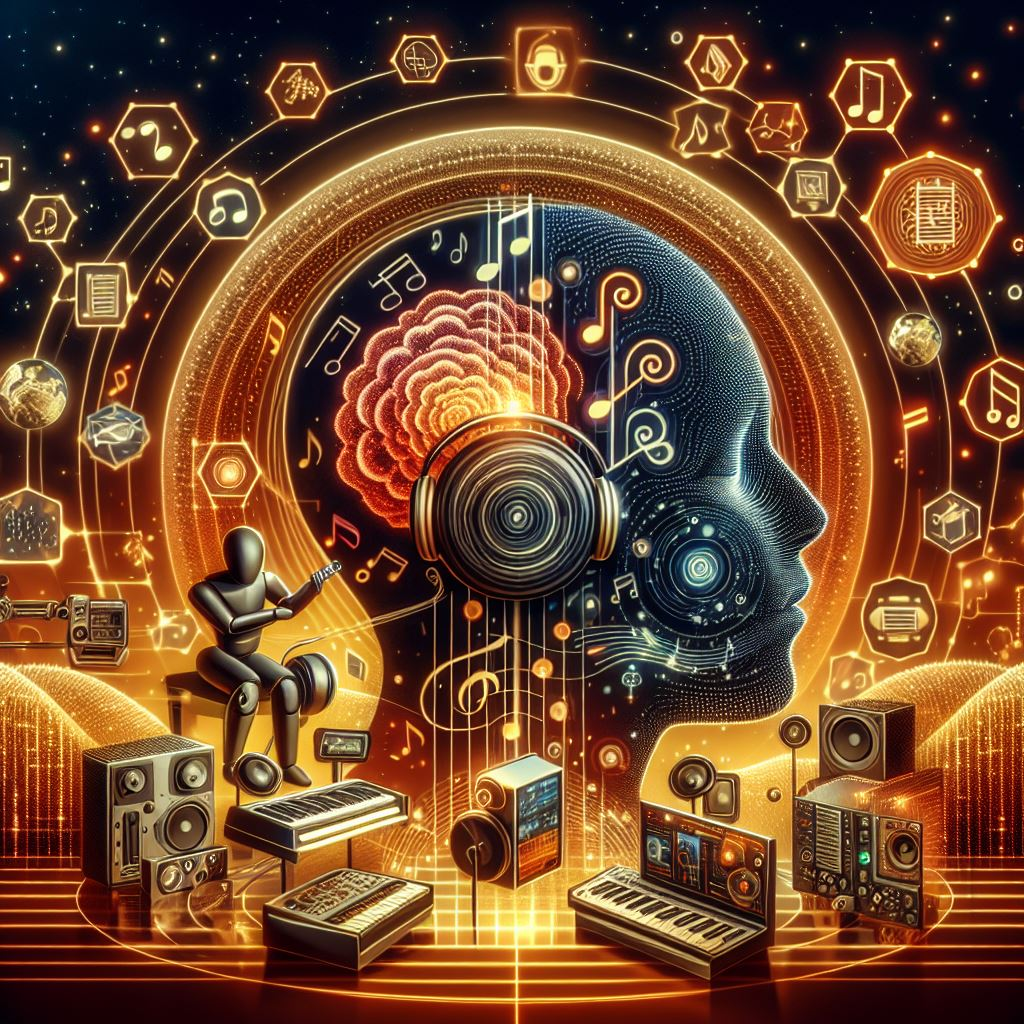
\includegraphics[width=.8\columnwidth]{musictech-apps}
						\end{figure}
		\end{columns}
    \inserticon{directions}
\end{frame}

